Problem 2: Larger unlabeled subset\\
Part 1: Visualization\\
Question 1.1:\\
\textsl{Provide at least one visualization which clearly shows the existence of the three main brain cell types described by the scientist, and explain how it shows this. Your visualization should support the idea that cells from a different group (for example, excitatory vs inhibitory) can differ greatly.}\\

Answer:\\
The dimensionality of the $log_2(X+1)$-transformed data can be reduced by using PCA. In this case we need a high amount of PC's to explain a satisfying variance (see \ref{fig:pcaanalysis}). For example, we need approximately 500 PC's to explain $60\%$ of the variance. Therefore, there is a high chance that data points can differ quite a lot within each cluster.

\begin{figure}[h]
	\centering
	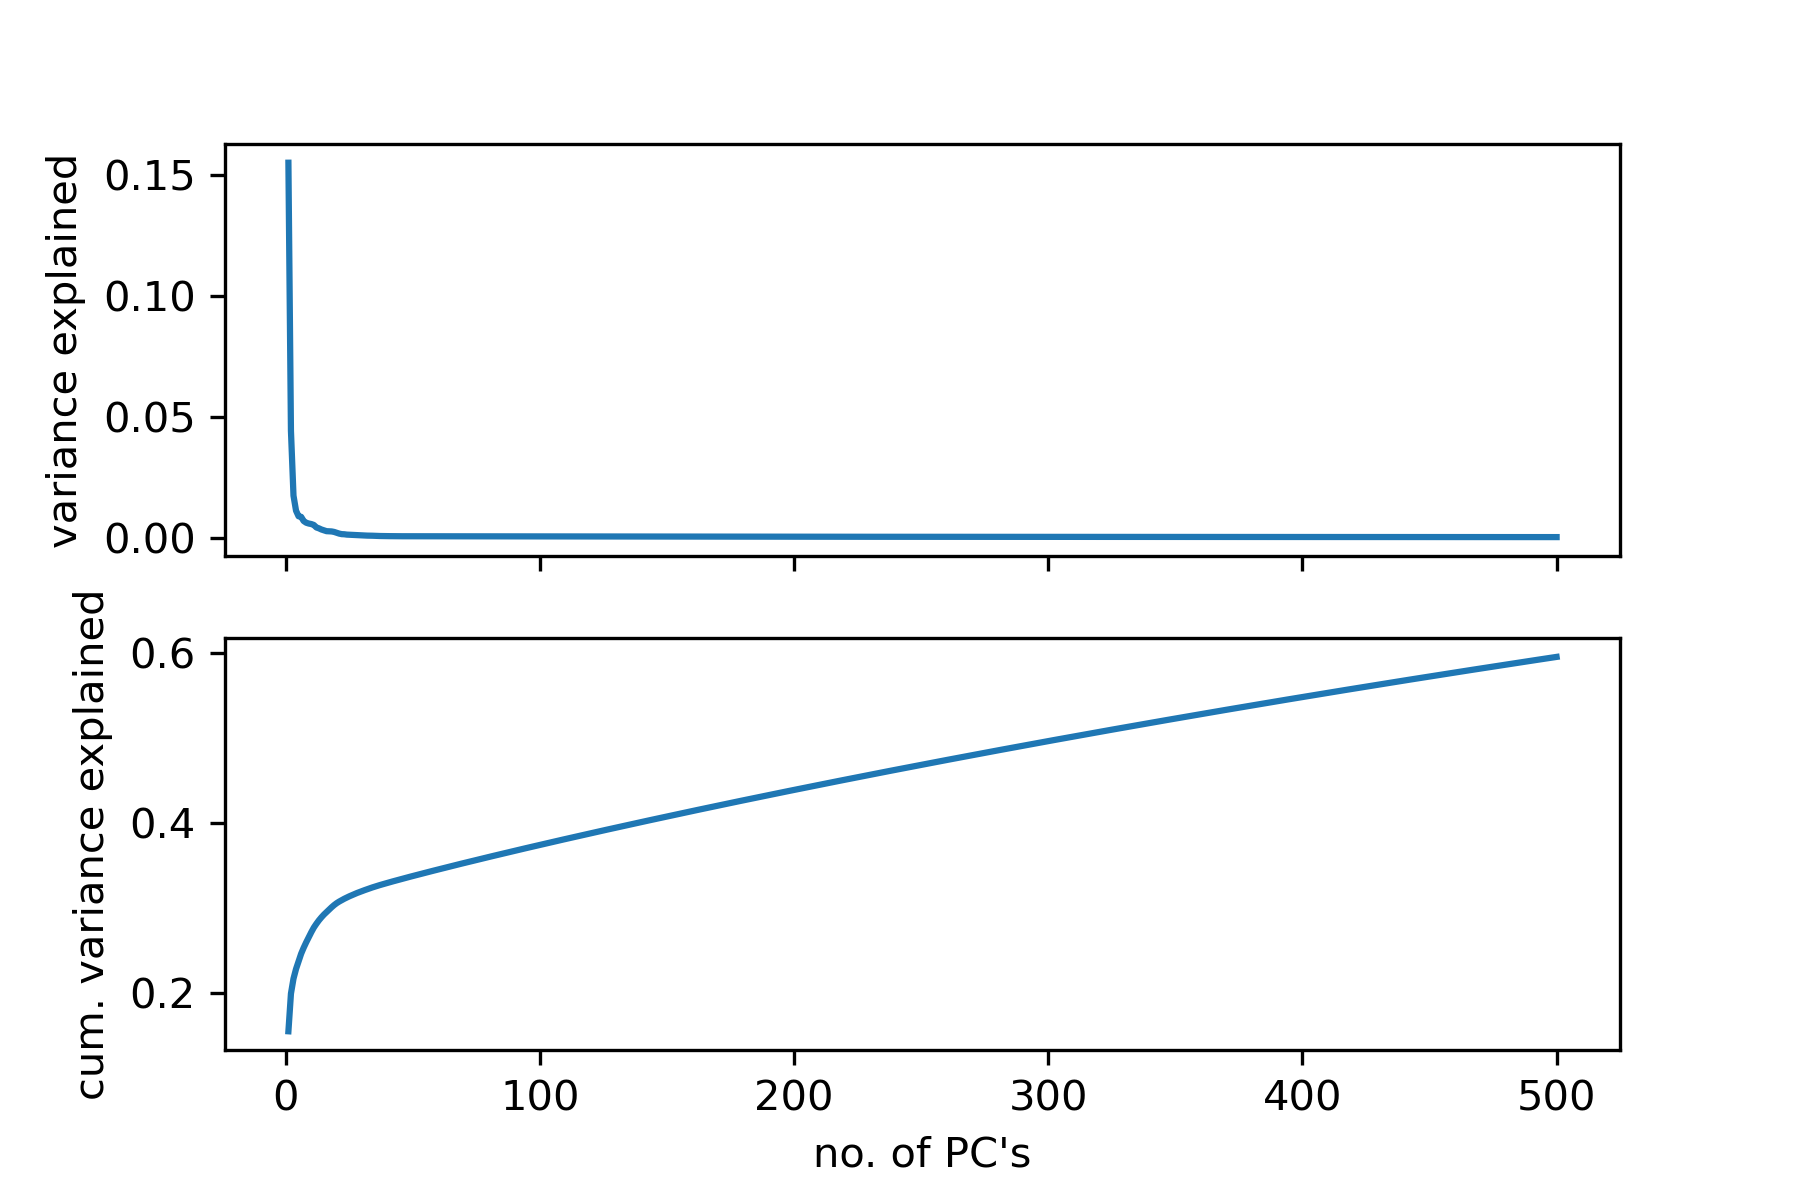
\includegraphics[width=0.6\linewidth]{problem_02/PCA_analysis}
	\caption{Variance explained (top) and cumulated variance explained (bottom)}
	\label{fig:pcaanalysis}
\end{figure}

%TODO: when there is more time: explain broadly how it works
For simplicity's sake, we only use 50 PC's to run the K-Means clustering function. Unfortunately, there is no set of labels corresponding to the data set. Therefore a comparison between the real cell types and the following shown clusters cannot be done. Nevertheless, the plot of the data can be split up into 3 clusters quite comfortably, which might be conform to three different cell types. This can either be done by plotting the data points over the first two PC's or be using T-SNE (see figure \ref{fig:clusters}).

\begin{figure}[h]
	\centering
	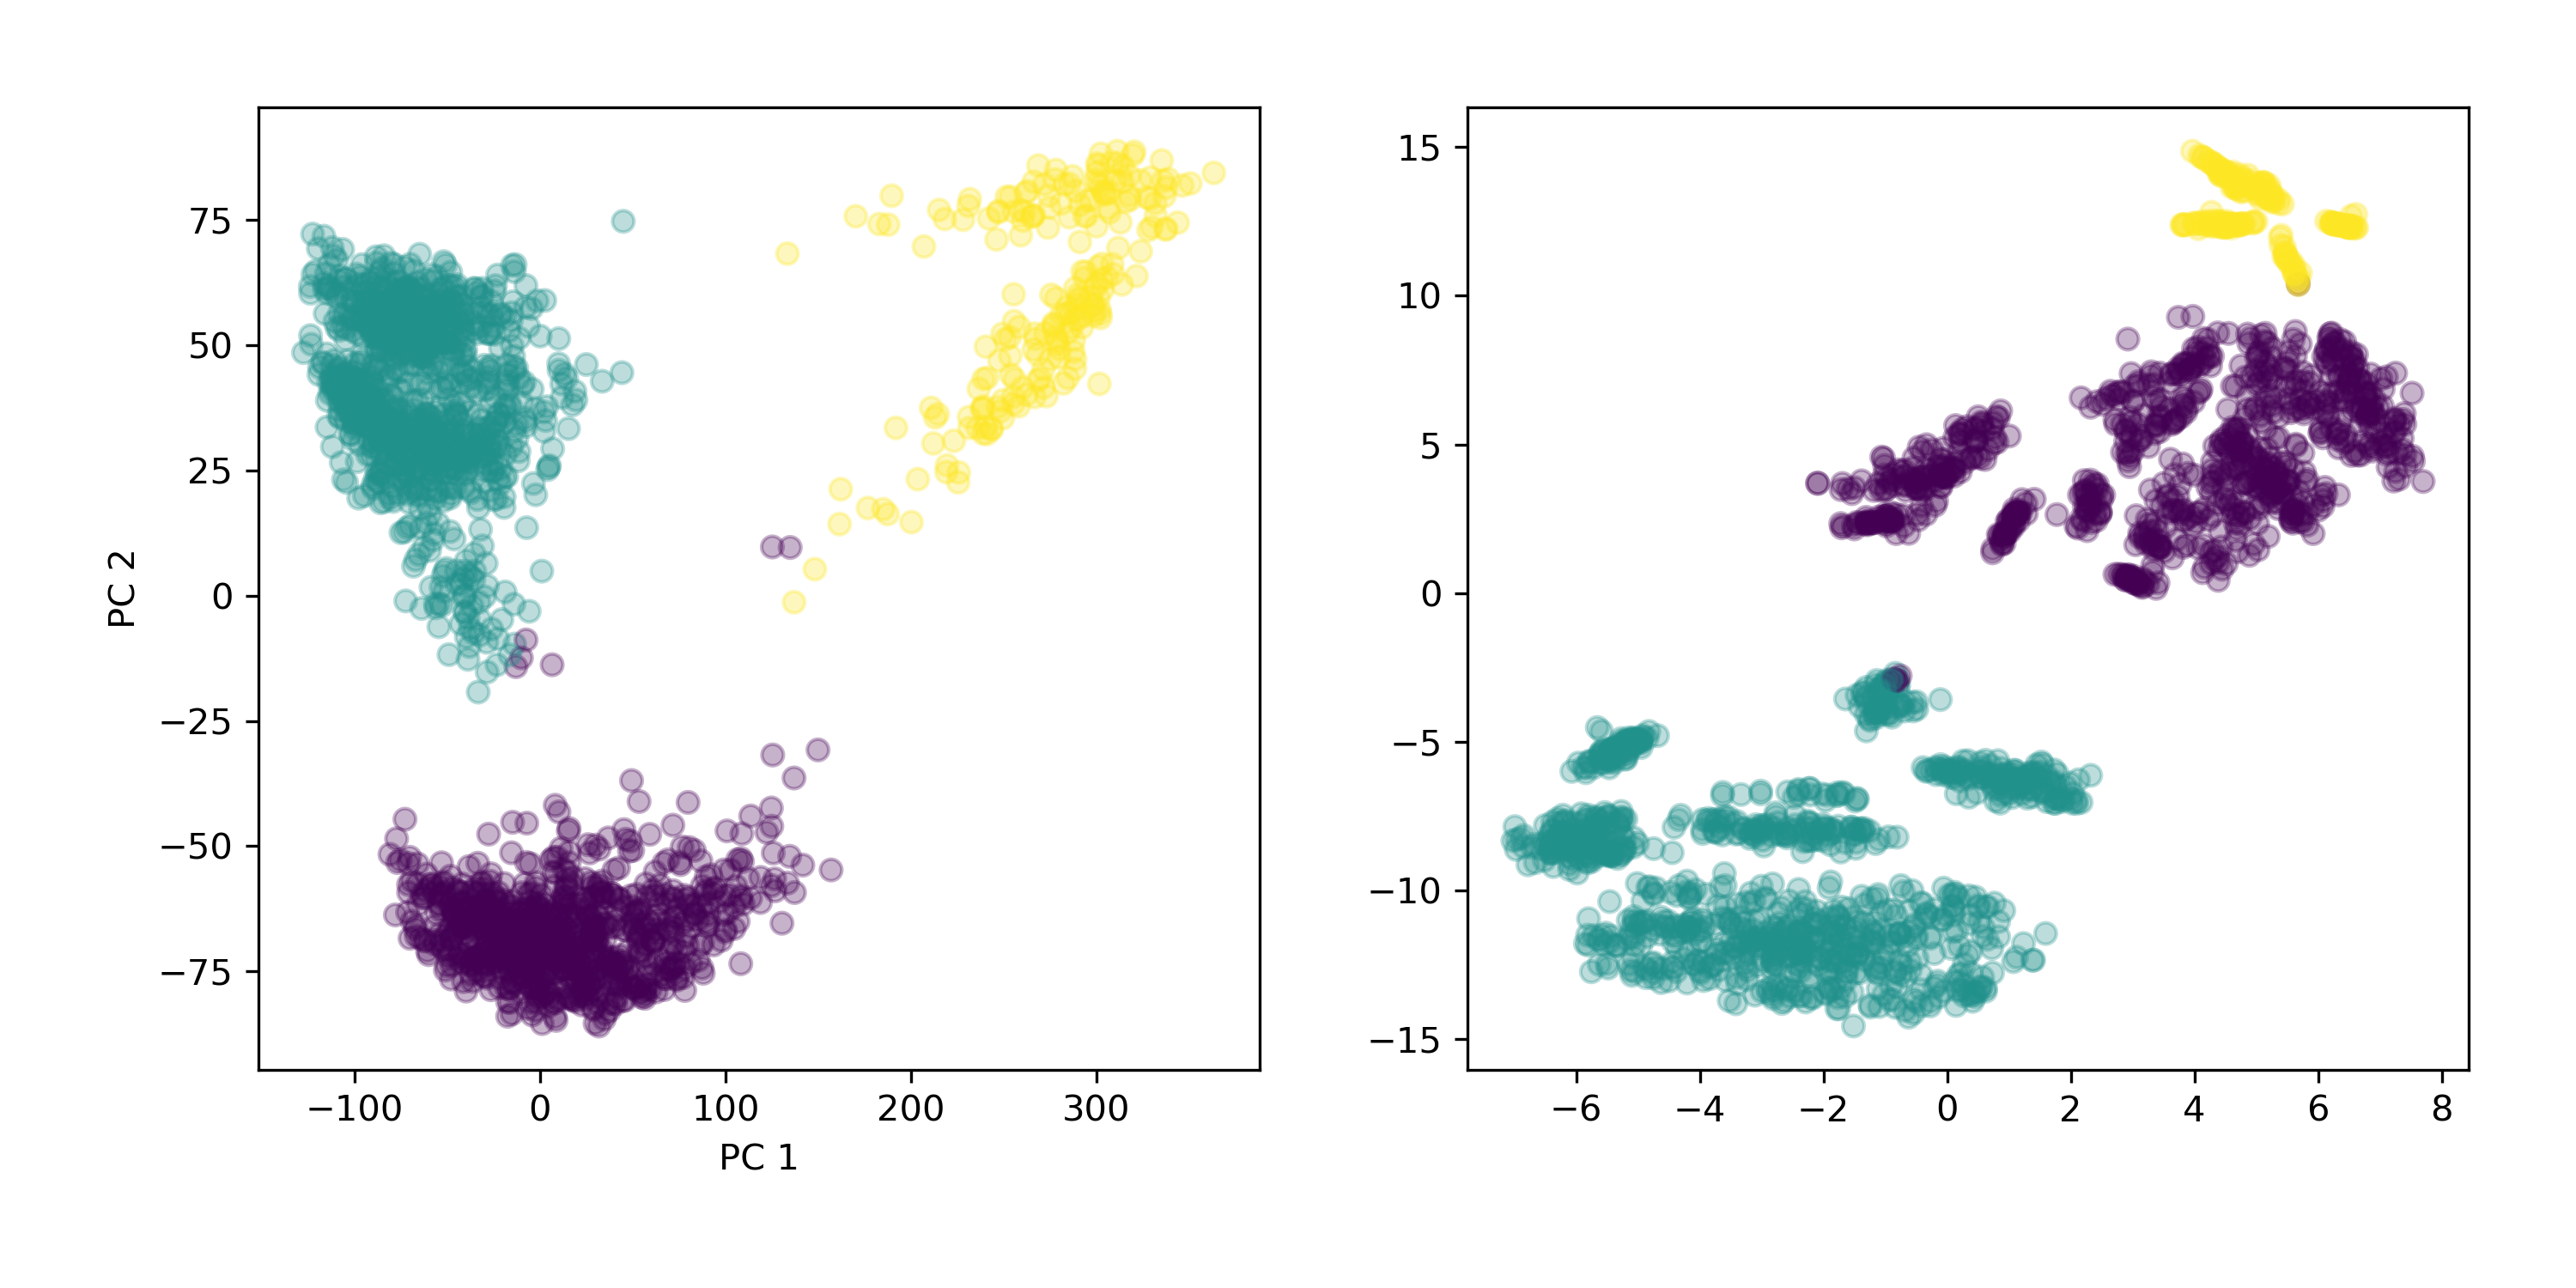
\includegraphics[width=0.9\linewidth]{problem_02/clusters}
	\caption{3 clusters (over first two PC's, left), 3 clusters (T-SNE (perplexity=500), right)}
	\label{fig:clusters}
\end{figure}